\documentclass[11pt]{article}

\usepackage{amsmath}
\usepackage{textcomp}
\usepackage[top=0.8in, bottom=0.8in, left=0.8in, right=0.8in]{geometry}
\usepackage{graphicx}
\usepackage{subcaption}
\usepackage{caption}
\usepackage{multirow}
% Add other packages here %


% Put your group number and names in the author field %
\title{\bf Excercise 4\\ Implementing a centralized agent}
\author{Group \textnumero 54: Oriol Barbany Mayor, Natalie Bolón Brun}


% N.B.: The report should not be longer than 3 pages %


\begin{document}
\maketitle

\section{Solution Representation}
\subsection{Variables}
% Describe the variables used in your solution representation %
The variables we chose are the pair of pickup and delivery actions derived from every task. This representation allows to perform multiple tasks at the same time. Note that in this representation, we say that more than one action is performed at a given time if the pair of pickup and delivery actions associated to the task are not consecutive.

\subsection{Constraints}
% Describe the constraints in your solution representation %
\begin{itemize}
    \item For each task, its pickup precedes the delivery.
    \item The total weight carried from any pickup action to its correspondent delivery, doesn't exceed the maximum capacity of the vehicle at any time in between.
    \item In case that a vehicle has a non-empty plan, its first action is a pickup.
    \item In any non-empty plan, the last action is a delivery.
\end{itemize}

\subsection{Objective function}
% Describe the function that you optimize %
For each vehicle, we keep track of the sequence of pickup and delivery actions performed as well as the plan associated to it. This latter involves pickups and deliveries but also moves that are introduced as the shortest path between such sequence of pickups and deliveries.

The \texttt{Plan} class implements a total distance function that we weight by the cost per kilometer of each vehicle. Then, the objective functions results by adding all these costs per vehicle.

Note that this doesn't take into account the time nor the distribution of tasks among all vehicles, so it can happen that an optimal plan only involves one vehicle or a few of them.

\section{Stochastic optimization}

\subsection{Initial solution}
% Describe how you generate the initial solution %
We generate the initial solution by distributing the tasks along the possible vehicles which have enough capacity to carry them. The tasks are performed sequentially, i.e. delivery and pickup pairs one after another and hence not picking up multiple tasks at the same time. In Section \ref{sec:experiment1} we study the influence of the initial solution. 

\subsection{Generating neighbours}
% Describe how you generate neighbors %
We generate neighbors by both transferring the first task of a given vehicle to another and permuting the set of tasks of a vehicle with the functions \texttt{changingVehicle} and \texttt{changingOrder} respectively.

\subsubsection{\texttt{changingVehicle}}
To create neighbors using this function, we first select uniformly at random one of the vehicles out of those that have tasks, say $v_i$. Then, for each other vehicle $v_j$, we append the first pickup of $v_i$ and the corresponding delivery to the beginning of $v_j$. As an example, let $p_1$ be the first action of $v_i$ (that is a pickup by the constraints) and $d_1$ its correspondent delivery. For a sequence of actions $v_i=[p_1, \mathbf{X},d_1,\mathbf{Y}]$ and $v_j=[\mathbf{Z}]$, we generate a neighbor $v_i=[\mathbf{X},\mathbf{Y}]$ and $v_j=[p_1, d_1, \mathbf{Z}]$.

Afterwards, we allocate both actions $p_1$ and $d_1$ inside the plan of vehicle $v_j$ with the function \texttt{changingOrder}.

\subsubsection{\texttt{changingOrder}}
This function gets a plan that starts with a pickup and delivery pairs that appear consecutively (recall output of \texttt{changingVehicle}). Then, it outputs all the possible feasible combinations (those satisfying the constraints) of inserting the pickup and the delivery inside the plan.


\subsection{Stochastic optimization algorithm}
% Describe your stochastic optimization algorithm %
We keep generating neighbors with the previous procedure and keep track of the best plan seen so far. Then, we explore the neighbors of a given potential solution following an $\varepsilon-$greedy policy, i.e. with probability $p$ we explore the neighbors of the best action and with probability $1-p$ we explore the neighbors of one random action among the potential solutions generated in a given iteration. In Section \ref{sec:experiment1} we further explain the details of the policy.

\section{Results}

\subsection{Experiment 1: Model parameters} \label{sec:experiment1}
% if your model has parameters, perform an experiment and analyze the results for different parameter values %
Comparison of performance of the $\varepsilon-$greedy policy with fixed or variable acceptance probability $p$. Comparison of different initial solutions. 

\subsubsection{Setting}
% Describe the settings of your experiment: topology, task configuration, number of tasks, number of vehicles, etc. %
% and the parameters you are analyzing %
The performance of each different policy is evaluated using the English topology with a total of 30 tasks and 4 vehicles with equal capacity (30kg) and cost per km (5u/km). 

The evaluated policies are $\varepsilon-$greedy with constant acceptance probability $p \in \{ 0.3, 0.5, 0.8\}$ and with variable probability $p$. For the evolution of $p$, we compare two different functions: 
$ p = 0.3 - 0.075 log(\frac{10}{i+1})$ and $ p = min(0.3+0.1 \frac{i}{75}, 0.9)$, with $i = $ number of iteration. Note that with the logarithmic increase, $p$ can go up to infinity, but we evaluate $X>p$ with $X\sim \mathcal{U}[0,1]$ so implicitly $p=\min(1,p)$, hence it remains a probability. Moreover we don't reach the equivalent of $p=1$ until iteration $\simeq130,000$.

For the initialization of the solution we compare the case in which all tasks are carried by a single vehicle and the case in which they are distributed among all possible vehicles.

\subsubsection{Observations}
% Describe the experimental results and the conclusions you inferred from these results %
In Figure \ref{fig:fixed-p} and \ref{fig:variable-p} we compare the quality of the solution for different policies, all initialized with a single vehicle carrying all tasks. 

\begin{minipage}{.4\textwidth}
\centering
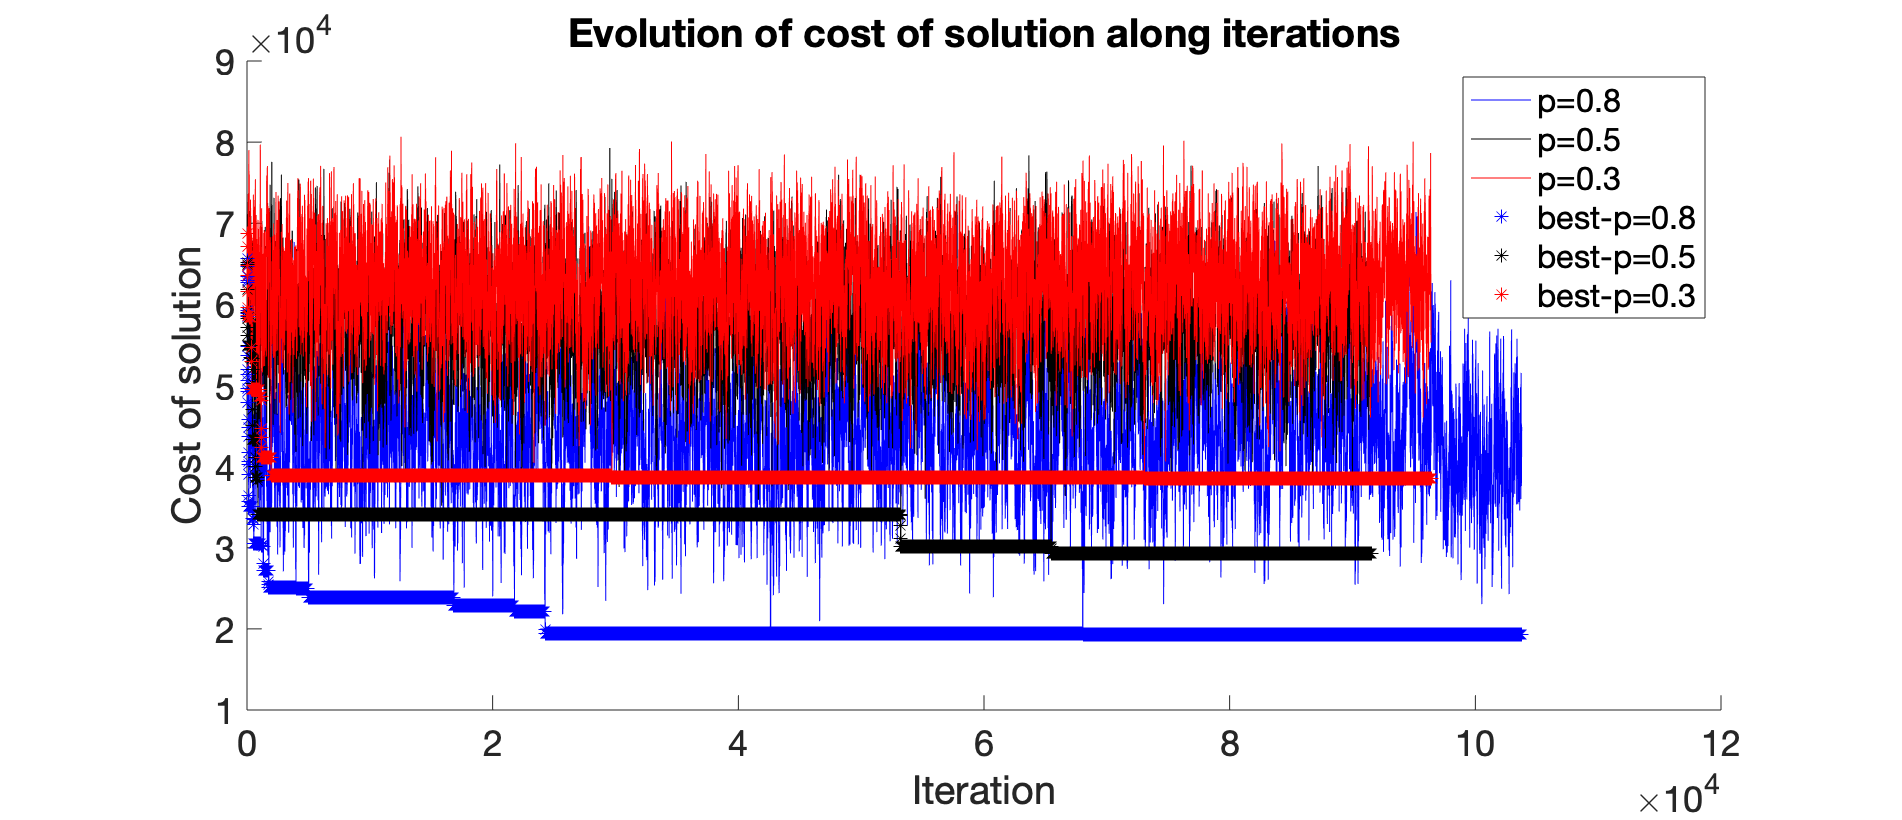
\includegraphics[width=\textwidth]{plots-centralized/evolution-fixed.png}
\captionof{figure}{Evolution of the cost along the iterative search with constant probability}
\label{fig:fixed-p}

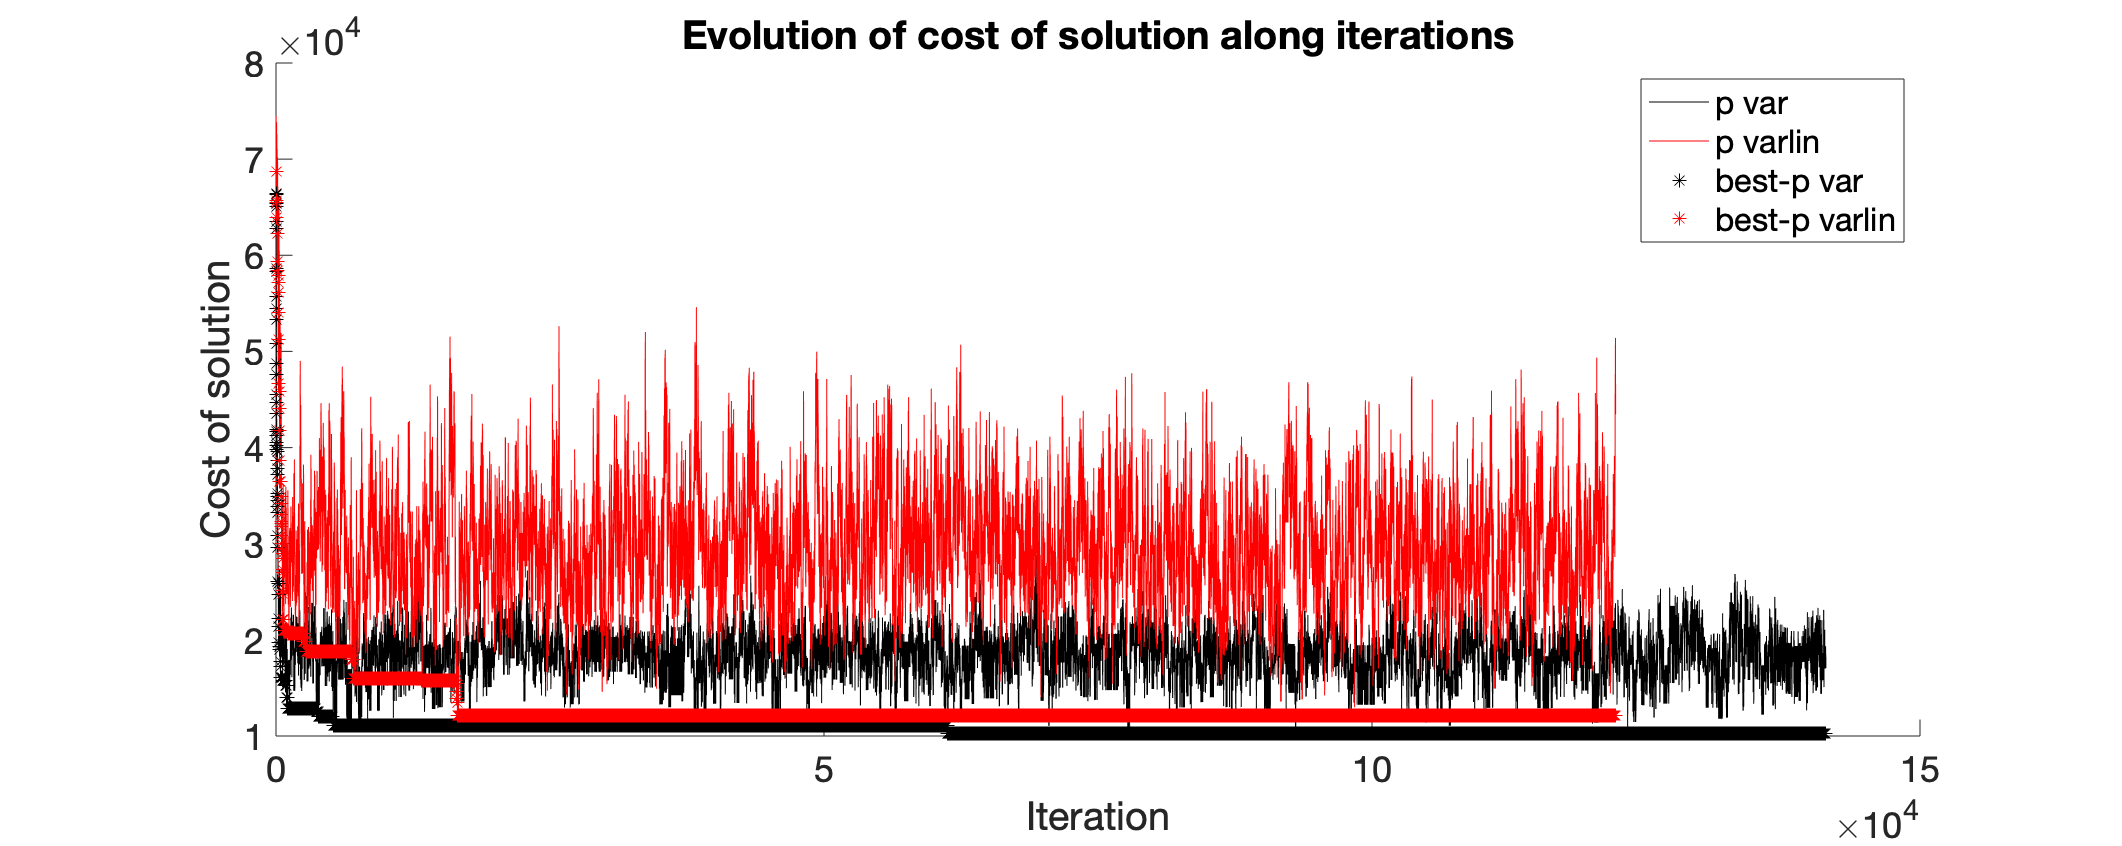
\includegraphics[width=\textwidth]{plots-centralized/evolution-variable.png}
\captionof{figure}{Evolution of the cost along the iterative search with variable probability}
\label{fig:variable-p}

\end{minipage}
\begin{minipage}{.6\textwidth}
While allowing a lower probability of refusing the optimal local solution helps the exploration of the space, it also slows down the convergence towards the optimal solution. We can see this trade off reflected in Figure \ref{fig:fixed-p}. For lower values of $p$ the cost of the selected solutions may vary a lot and the improvements are made at lower pace. On the other hand, higher $p$ provides fast improvement but gets stuck in a local optima. We can see that in this case the solution does not make any improvement after 19000 iterations (out of $\simeq 126000$ iterations).

In order to combine the best of both behaviours, we use a variable value for $p$. Figure \ref{fig:variable-p} shows the evolution of the cost of the solution with $p$ varying linearly or in a logarithmic fashion. We can see the best result is achieved by applying a logarithmic variation to the greediness of the policy. The best solution obtained has a cost of 10249u. The best solution obtained by an $\varepsilon-$greedy policy with fixed $\varepsilon$ increases the cost by an 88\%. 

Regarding the influence of the initialization, using the multiple vehicle initialization results in a worse performance when using the fixed $\varepsilon$ policy, increasing the final cost by a 10\% in average. On the other hand, this initialization performs better with the variable policy, reducing the \textbf{best obtained cost to 9989u}  

\end{minipage}


\subsection{Experiment 2: Different configurations}
% Run simulations for different configurations of the environment (i.e. different tasks and number of vehicles) %
In this section, we perform different experiments varying the number of vehicles, tasks and characteristics of the vehicles. The time to generate the solution is set to 30s in all cases. 

\subsubsection{Setting}
The following simulations are performed on the English topology. We test all the possible tuples $(n_{veh},n_{tasks},f)$, where $n_{veh} \in \{1, 3, 6\}$,  $n_{tasks} \in \{ 5, 20, 50\}$ and $f\in \{H_o,H_e\}$, which stands for homogeneous and heterogeneous fleet of vehicles. Note that there's no notion of fleet with one vehicle. We use the $\varepsilon-$greedy policy with logarithmic evolution of $p$ and multiple vehicle initialization.
% Describe the settings of your experiment: topology, task configuration, number of tasks, number of vehicles, etc. %

\subsubsection{Observations}
% Describe the experimental results and the conclusions you inferred from these results %
% Reflect on the fairness of the optimal plans. Observe that optimality requires some vehicles to do more work than others. %
% How does the complexity of your algorithm depend on the number of vehicles and various sizes of the task set? %
\begin{minipage}{0.35\textwidth}
\resizebox{\textwidth}{!}{%
\begin{tabular}{|c|c|c|c|c|}
\hline
num. vehicles & fleet type & \multicolumn{3}{c|}{num. tasks} \\ \hline
 &  & \textbf{5} & \textbf{20} & \textbf{50} \\ \hline
\textbf{1} & - & 7262 & 16106 & 123297 \\ \hline
\multirow{2}{*}{\textbf{3}} & $H_o$ & 5053 (1) & 9199.5 (1) &  17751 (1)\\ \cline{2-5} 
 & $H_e$ & 5053 (1) & 11385.5 (1) &  29242 (1) \\ \hline
\multirow{2}{*}{\textbf{6}} & $H_o$ & 5053 (1)  & 9774.5 (1) & 16732 (1) \\ \cline{2-5} 
 & $H_e$ & 3220 (1) & 11922.6 (3) & 18378.0 (2) \\ \hline
\end{tabular}%
}
\captionof{table}{Cost obtained after 30s.\\(i) = Num used vehicles.}
\label{tab:configurations}
\end{minipage}{}
\hfill
\begin{minipage}{0.6\textwidth}
In terms of complexity of the algorithm, the computations per iteration are proportional to the number of neighbors, which grows as $\mathcal{O}(n_{tasks}^2 n_{veh})$, since for all vehicles but one (the previously called $v_i$), we explore the set of feasible permutations of a new pickup and delivery pair. The cardinality of this latter is $\mathcal{O}(n_{tasks}^2)$ due to the constraints.


\end{minipage}

When using a heterogeneous fleet, the best solution tends to use a single vehicle, selecting the one with lower cost (and maximum capacity if there is more than one with the same cost). If we lower the cost and limit capacities (max. one task per vehicle), the optimal solution is forced to be one including multiple vehicles. 

To sum up, we see that the optimal plans tend to exploit solutions with a single vehicle (or a few) since when carrying a task, the vehicle already visits other cities along the path where there can be other tasks. Exploiting the option of carrying multiple tasks is enough to reduce the cost and, as stated before, we are not penalizing the time for the completion of the tasks nor directly rewarding the even distribution of tasks.

%% limit capacity of vehicles --> limit feasible set
%% increase vehicles --> 

\end{document}